\documentclass[12pt,spanish]{article}
\usepackage[spanish]{babel}
\usepackage[utf8]{inputenc}
\usepackage[hyphens]{url}
\usepackage[margin=0.75in]{geometry}
\usepackage{float}
\usepackage{placeins}
\usepackage{graphicx}
\usepackage[nottoc, notlot, notlof, notindex]{tocbibind}
\usepackage{tocloft}
\usepackage[colorlinks,bookmarksopen]{hyperref}
\renewcommand{\cftsecleader}{\cftdotfill{\cftdotsep}}
\newcommand{\quotes}[1]{``#1''}
\selectlanguage{spanish}
\title{\textbf{Migración de una aplicación a Kubernetes}}
\author{Israel Pavón Maculet\\
  \and
  Sergio Arroutbi Braojos}
\date{\today}
\begin{document}

\maketitle

\tableofcontents

\listoffigures

\section{Introducción}

Para esta práctica se ha utilizado, como aplicación distribuida de base para la práctica, el proyecto conocido como ``Guardarpunto''. Esta aplicación esta disponible en el siguiente enlace de Github:\\

\url{https://github.com/mfms5/guardarpunto/}\\

En cuanto a realizar la implementación de los diversos ficheros que permitan el despliegue de dicha aplicación en un entorno basado en el sistema de orquestación de contenedores Kubernetes, se ha optado por realizar un ``fork'' del proyecto anterior en el siguiente repositorio de ``github'':\\

\url{https://github.com/sarroutbi/guardarpunto}\\

El repositorio anterior, básicamente, contiene una serie de carpetas adicionales respecto al proyecto original que se enumeran a continuación:

\begin{enumerate}
\item{\textbf{docker} :} Esta carpeta contiene los ficheros Dockerfile que permiten la construcción de los distintos contenedores que sustituyen a las máquinas virtuales del proyeto original.
\item{\textbf{helm} :} Bajo este directorio aparecen los ficheros necesarios para realizar el despliegue basado en \textbf{helm}, el gestor de paquetes de Kubernetes que permite
\item{\textbf{doc} :} Contiene los ficheros necesarios para la elaboración de la presente documentación.
\end{enumerate}

En cuanto a las tecnologías utilizadas, el despliegue se ha basado, como ya se comentó anteriormente, en \textbf{helm} como gestor de paquetes de Kubernetes. Por otra parte, como sistema base Kubernetes se ha optado por \textbf{minikube}.

En la sección~\ref{sec:deployment} se realizará una descripción detallada del despliegue realizado, así como de los pasos seguidos para generar los contenedores apropiados que sustituyan a las máquinas virtuales originales de la aplicación (``dockerización'') así como los ficheros helm que permiten el despliegue y orquestación de dichos contenedores de aplicación en la infraestructura Kubernetes.

\section{Descripción del despliegue en Kubernetes}
\label{sec:deployment}

\subsection{Despliegue}

TODO: Descripción del despliegue: Servicios, Deployments, Pods, Ingress.
%\begin{center}
% \begin{figure}[H]
% \begin{center}
%   \includegraphics[width=17cm]{img/deployment00.png}
%   \caption{Despliegue de aplicación}
%   \label{fig:deployment00}
% \end{center}
% \end{figure}
%\end{center}

\subsection{Docker}

En cuanto a la generación de los contenedores, se ha creado una carpeta ``docker'' en la raíz del proyecto descrito anteriormente. Dicha carpeta contiene diversos subdirectorios con los distintos contenedores que se han utilizado como sustitución de las máquinas virtuales del proyecto inicial, y que se enumeran a continuación:

\begin{itemize}
\item{\textbf{webfront1}}. Esta carpeta contiene el Dockerfile necesario para, partiendo de una imagen base Ubuntu 14.04 (la utilizada en el proyecto original), instalar el JDK de Java 8 apropiado, clonar el código de la aplicación frontal web y recoger las instrucciones de arranque de la misma. Se ha optado por hacer una aplicación principal con un POD distinto al otro frontal web por el hecho de que en la aplicación original las opciones de arranque y el usuario a utilizar son distintos respecto a la aplicación secundaria / backup.
A continuación se incluye el \textbf{``Dockerfile''} utilizado:
\begin{verbatim}
# Pull base image
FROM ubuntu:14.04

# Variables
ENV REPOSITORY https://github.com/sarroutbi/guardarpunto.git
ENV WEB_APP_PATH guardarpunto/guardar_punto_2/target/
guardar_punto-0.0.1-SNAPSHOT.jar
ENV JAVA_HOME /usr/lib/jvm/java-8-oracle
ENV PATH $PATH:$JAVA_HOME/bin

# Update latest software and install java modules
# software-properties-common needed for add-apt-repository command
RUN sudo apt-get update && \
    sudo apt-get install -y git && \
    sudo apt-get install -y software-properties-common && \
    sudo apt-add-repository ppa:webupd8team/java && \
    sudo add-apt-repository ppa:openjdk-r/ppa && \
    sudo apt-get update && \
    echo "oracle-java8-installer shared/accepted-oracle-license-v1-1 select true" \
    | sudo debconf-set-selections && \
    sudo apt-get install -y oracle-java8-installer && \
    sudo apt-get install -y openjdk-8-jre

# Clone software source and copy bin file to this path
RUN git clone -v ${REPOSITORY} && \
    cp -v ${WEB_APP_PATH} .

# Run web application
# TODO: Parametrize IPs, usernames, passwords, etc
CMD ["java", "-jar",
     "guardarpunto/guardar_punto_2/target/guardar_punto-0.0.1-SNAPSHOT.jar",
     "--spring.datasource.url=jdbc:mysql://mysqlsrv:3306/guardarpuntodb?
verifyServerCertificate=false&useSSL=true",
     "--spring.datasource.username=user1",
     "--spring.datasource.password=enjutomojamuto",
     "--spring.jpa.hibernate.ddl-auto=create"]
\end{verbatim}
\item{\textbf{webfront2}}. Esta carpeta contiene el Dockerfile necesario para generar una aplicación similar a la anterior, pero con las opciones de arranque cambiadas según estaban en el proyecto original (distinto usuario de conexión a base de datos y distintas opciones de arranque de la aplicación Spring Boot):
A continuación se incluye el \textbf{``Dockerfile''} utilizado:
\begin{verbatim}
# Pull base image
FROM ubuntu:14.04

# Variables
ENV REPOSITORY https://github.com/sarroutbi/guardarpunto.git
ENV WEB_APP_PATH guardarpunto/guardar_punto_2/target/guardar_punto-0.0.1-SNAPSHOT.jar
ENV JAVA_HOME /usr/lib/jvm/java-8-oracle
ENV PATH $PATH:$JAVA_HOME/bin

# Update latest software and install java modules
# software-properties-common needed for add-apt-repository command
RUN sudo apt-get update && \
    sudo apt-get install -y git && \
    sudo apt-get install -y software-properties-common && \
    sudo apt-add-repository ppa:webupd8team/java && \
    sudo add-apt-repository ppa:openjdk-r/ppa && \
    sudo apt-get update && \
    echo "oracle-java8-installer shared/accepted-oracle-license-v1-1 select true" \
| sudo debconf-set-selections && \
    sudo apt-get install -y oracle-java8-installer && \
    sudo apt-get install -y openjdk-8-jre

# Clone software source and copy bin file to this path
RUN git clone -v ${REPOSITORY} && \
    cp -v ${WEB_APP_PATH} .

# Run web application
# TODO: Parametrize IPs, usernames, passwords, etc
CMD ["java", "-jar",
     "guardarpunto/guardar_punto_2/target/guardar_punto-0.0.1-SNAPSHOT.jar",
     "--spring.datasource.url=jdbc:mysql://mysqlsrv:3306/guardarpuntodb?
verifyServerCertificate=false&useSSL=true", "--spring.datasource.username=user2",
     "--spring.datasource.password=enjutomojamuto"]
\end{verbatim}
\item{\textbf{mysqlsrv}}. Bajo este directorio se encuentra el Dockerfile necesario para generar el contenedor de base de datos, partiendo de una versión de Ubuntu 14.04, de igual forma que en la práctica original, y con las opciones de instalación de la base de datos utilizada (``mysql'' en este caso), creación de la base de datos, configuración de usuarios, privilegios de los mismos, tablas necesarias y parámetros de conexión necesarios, a parte de las distintas personalizaciones necesarias para este tipo de aplicaciones, como pueda ser el ajuste de la dirección a la que hacer ``bind'', exposición de los puertos utilizados por mysql, etc.
A continuación se incluye el \textbf{``Dockerfile''} utilizado:
\begin{verbatim}
# Pull base image
FROM ubuntu:14.04

# Update latest software and install java modules
# software-properties-common needed for add-apt-repository command
RUN sudo apt-get update && \
    sudo rm -fr /var/lib/mysql && \
    sudo mkdir -p /mnt/mysql/data && \
    sudo ln -s /mnt/mysql/data /var/lib/mysql && \
    sudo apt-get -q -y install mysql-server && \
    sudo apt-get install -y software-properties-common && \
    sudo apt-add-repository ppa:openjdk-r/ppa && \
    sudo apt-get update && \
    sudo apt-get install -y openjdk-8-jre && \
    sudo sed -i 's/^bind-address/#bind-address/' /etc/mysql/my.cnf && \
    sudo service mysql start && \
    mysql -u root -e \
     "CREATE DATABASE guardarpuntodb;\
     create user 'user1'@'localhost' identified by 'enjutomojamuto';\
     create user 'user2'@'localhost' identified by 'enjutomojamuto';\
     grant all on guardarpuntodb.* to 'user1'@'localhost'\
identified by 'enjutomojamuto';\
     grant all on guardarpuntodb.* to 'user2'@'localhost'\
identified by 'enjutomojamuto';\
     grant all on guardarpuntodb.* to 'user1'@'%'\
identified by 'enjutomojamuto';\
     grant all on guardarpuntodb.* to 'user2'@'%'\
identified by 'enjutomojamuto';\
     flush privileges;"

COPY start_mysql.sh /usr/bin

# Start with just a shell, mysql will be running appropriately
EXPOSE 3306 33060
CMD ["/usr/bin/start_mysql.sh"]
\end{verbatim}
Como puede verse anteriormente, además del fichero ``Dockerfile'', bajo esta carpeta se encuentra también un sencillo script ``start\_mysql.sh'', que realiza, básicamente, dos operaciones:
\begin{itemize}
\item{Copiar, en primer arranque, los ficheros de base de datos al directorio definido para almacenamiento permanente a través de PVC}.
\item{Arrancar la base de datos con las opciones necesarias en cuanto a resolución de nombres y directorio de datos utilizado}.
\end{itemize}
A continuación se muestra el contenido del script de arranque de la base de datos, ``start\_mysql.sh'':
\begin{verbatim}
#!/bin/bash
# 1 - Copy data to pvc disk if it is the first time
test -f /mnt/data/copied
if [ $? -eq 1 ];
then
  cp -arfv /var/lib/mysql/ /mnt/data/
  touch /mnt/data/copied
fi

# 2 - Start database
mysqld --skip-name-resolve --datadir=/mnt/data/mysql/
\end{verbatim}

\item{\textbf{internalsvc}}. Finalmente, un directorio que engloba el fichero ``Dockerfile'' necesario para generar el contenedor utilizado para la aplicación que sirve como servicio interno. En este caso, se trata de un servicio de mail que permite el envío de correos en el proceso de registro. Partiendo de una imagen base Ubuntu 14.04 (la utilizada en el proyecto original), instalar el JDK de Java 8 apropiado, clonar el código de la aplicación interna y recoger las instrucciones de arranque de la misma. A continuación se incluye el \textbf{``Dockerfile''} utilizado:
\begin{verbatim}
# Pull base image
FROM ubuntu:14.04

# Variables
ENV REPOSITORY https://github.com/sarroutbi/guardarpunto.git
ENV INTERNAL_SRVC_PATH
    ./guardarpunto/MailRestPost/target/MailRestPost-0.0.1-SNAPSHOT.jar
ENV JAVA_HOME /usr/lib/jvm/java-8-oracle
ENV PATH $PATH:$JAVA_HOME/bin

# Update latest software and install java modules
# software-properties-common needed for add-apt-repository command
RUN sudo apt-get update && \
    sudo apt-get install -y git && \
    sudo apt-get install -y software-properties-common && \
    sudo apt-add-repository ppa:webupd8team/java && \
    sudo add-apt-repository ppa:openjdk-r/ppa && \
    sudo apt-get update && \
    echo "oracle-java8-installer shared/accepted-oracle-license-v1-1 select true" \
| sudo debconf-set-selections && \
    sudo apt-get install -y oracle-java8-installer && \
    sudo apt-get install -y openjdk-8-jre

# Clone software source
RUN git clone -v ${REPOSITORY} && pwd && \
    cp -v ${INTERNAL_SRVC_PATH} .

# Run web application
# TODO: Substitue ile with INTERNAL_SRVC_PATH env variable
CMD ["java", "-jar",
     "./guardarpunto/MailRestPost/target/MailRestPost-0.0.1-SNAPSHOT.jar"]
\end{verbatim}

\end{itemize}

\subsection{Helm}

\section{Instrucciones para el despliegue de la aplicación}
\label{sec:instructions}

\subsection{Instrucciones paso a paso}
\begin{itemize}
\item{\textbf{Configuración del /etc/hosts}}. Con motivo de acceder a la aplicación distribuida de forma externa a través de nginx, se ha de configurar una dirección de host, en concreto ``guadarpunto.example.com'' en el ``/etc/hosts'' de la máquina, configurando la IP de minikube como IP de destino. para ello:
  \begin{itemize}
  \item{Consultar la IP de minikube}:
  \begin{verbatim}
  $ minikube ip
  192.168.99.100
  \end{verbatim}
  \item{Editar el fichero ``/etc/hosts'' para que contenga el nombre de dominio apropiado}:
  \begin{verbatim}
  $ head /etc/hosts
  192.168.99.100  guardarpunto.example.com
  ...
  \end{verbatim}
  \end{itemize}
\item{\textbf{Creación del directorio asociado a PVC}}. Para que los datos de la base de datos sean permanetes, se deberá crear un directorio determinado, /mnt/data, en el host, en este caso, en minikube. Por lo tanto:
  \begin{itemize}
  \item{Acceder a minikube por ssh y crear el directorio /mnt/data}:
  \begin{verbatim}
    $ minikube ssh
                             _             _
                _         _ ( )           ( )
      ___ ___  (_)  ___  (_)| |/')  _   _ | |_      __
    /' _ ` _ `\| |/' _ `\| || , <  ( ) ( )| '_`\  /'__`\
    | ( ) ( ) || || ( ) || || |\`\ | (_) || |_) )(  ___/
    (_) (_) (_)(_)(_) (_)(_)(_) (_)`\___/'(_,__/'`\____)

    $ mkdir /mnt/data/
    $ exit
    logout
  \end{verbatim}
  En el caso que el directorio /mnt/data estuviese ya creado, se ruega borrar por completo y recrearlo para evitar problemas en el arranque de la base de datos.
  \end{itemize}
\item{\textbf{Clonar el código de la aplicación}}:
\begin{verbatim}
$ git clone https://github.com/sarroutbi/guardarpunto.git
\end{verbatim}
\item{\textbf{Acceder a la raíz del proyecto, y desplegar la aplicación con ``helm''}}:
\begin{verbatim}
$ cd guardarpunto
$ helm install --name guardarpunto helm/guardarpunto/
\end{verbatim}
Posteriormente, comprobar que los diversos PODs se encuentran arrancados:
\begin{verbatim}
$ kubectl get pods
NAME                           READY     STATUS    RESTARTS   AGE
internalsvc-5479b96564-jzhz6   1/1       Running   0          19m
internalsvc-5479b96564-s4xmp   1/1       Running   0          19m
mysqlsrv-845b6cd78b-s9bqn      1/1       Running   0          19m
webfront1-95d579447-vj2xt      1/1       Running   0          19m
webfront2-5787f49c88-d5m4v     1/1       Running   0          19m
\end{verbatim}
\textbf{NOTA: La primera vez que se despliegue la aplicación, los contenedores se bajarán de forma completa desde dockerhub, luego se tardará varios minutos hasta que los pods estén desplegados.}
\item{\textbf{Acceder con el navegador a la página principal del proyecto: \url{http://guardarpunto.example.com}}}:
Deberá observarse una imagen similar a la que se muestra a continuación:
\begin{center}
 \begin{figure}[H]
 \begin{center}
   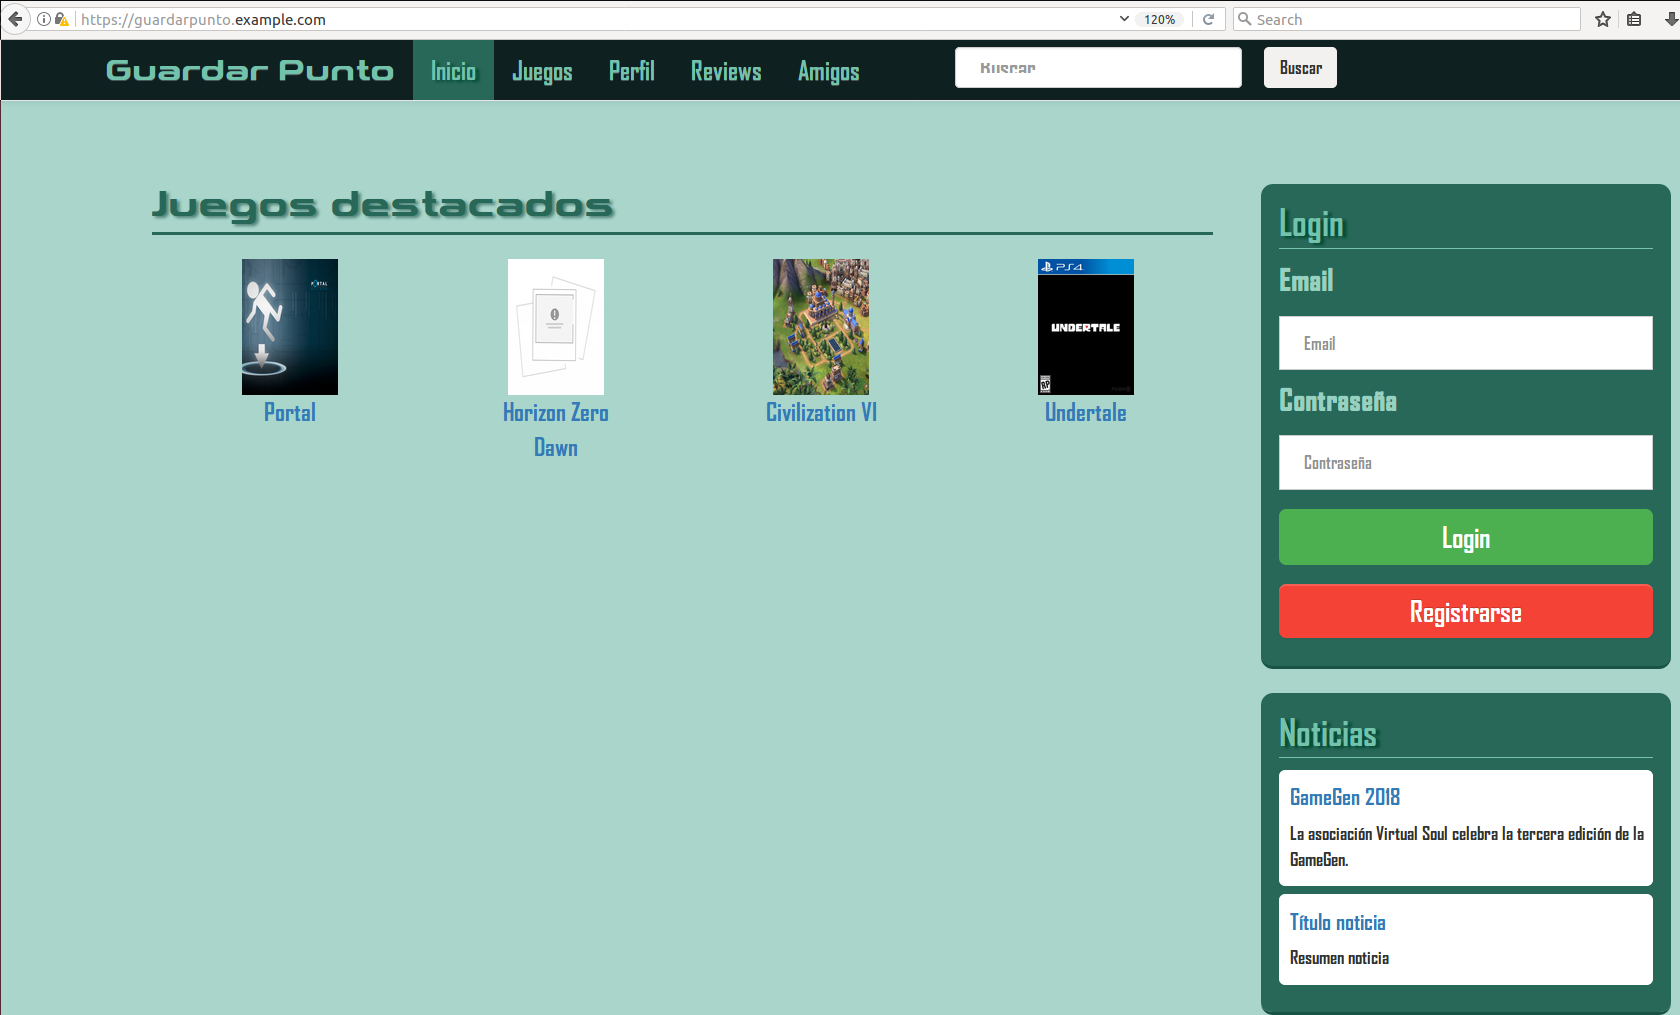
\includegraphics[width=17cm]{img/web01.png}
   \caption{Página de inicio}
   \label{fig:initpage00}
 \end{center}
 \end{figure}
\end{center}

\end{itemize}

\subsection{Descripción de software}
Con motivo de depurar posibles problemas en el despliegue, se enumeran las diferentes herramientas software utilizadas para posibilitar el despliegue en kubernetes:

\begin{enumerate}
\item{\textbf{minikube}:} Como herramienta de despliegue de un cluster mínimo de kubernetes. La versión utilizada ha sido la siguiente: \textbf{v0.35.0}.
  En cuanto a los ``addons'' de aplicación habilitados, se encuentran los siguientes:
\begin{verbatim}
  $ minikube addons list
  - addon-manager: enabled
  - dashboard: disabled
  - default-storageclass: disabled
  - efk: disabled
  - freshpod: disabled
  - gvisor: disabled
  - heapster: disabled
  - ingress: enabled
  - logviewer: disabled
  - metrics-server: disabled
  - nvidia-driver-installer: disabled
  - nvidia-gpu-device-plugin: disabled
  - registry: disabled
  - registry-creds: disabled
  - storage-provisioner: enabled
  - storage-provisioner-gluster: disabled
\end{verbatim}

\item{\textbf{helm}:} Como herramienta de gestión de paquetes en kubernetes. La versión utilizada ha sido la siguiente, tanto para cliente como para servidor: \textbf{v2.11.0}.
\begin{verbatim}
  $ helm version
  Client: &version.Version{SemVer:''v2.11.0'', GitCommit:''2e55dbe''}
  Server: &version.Version{SemVer:''v2.11.0'', GitCommit:''2e55dbe''}
\end{verbatim}

\item{\textbf{docker}:} Como herramienta de gestión de contenedores. La versión utilizada ha sido la siguiente, tanto para cliente como para servidor: \textbf{18.06.1-ce}.
\begin{verbatim}
Client:
 Version:           18.06.1-ce
 API version:       1.38
 Go version:        go1.10.3
 Git commit:        e68fc7a
 Built:             Tue Aug 21 17:24:56 2018
 OS/Arch:           linux/amd64
 Experimental:      false

Server:
 Engine:
 Version:          18.06.1-ce
 API version:      1.38 (minimum version 1.12)
 Go version:       go1.10.3
 Git commit:       e68fc7a
 Built:            Tue Aug 21 17:23:21 2018
 OS/Arch:          linux/amd64
 Experimental:     false
\end{verbatim}

\end{enumerate}

\end{document}
